\section{Experimental Results}
\label{sec:ExperimentalResults}
For a detailed description of all experimental settings and hyperparameters, see Appendix~\ref{appendix: Experiments}. The code for all the experiments can be found online at \url{https://github.com/bumsu-kim/CARS}.

 
\subsection{Convex Functions}
We compared the performance of CARS and CARS-CR to STP \cite{bergou2020stochastic}, SMTP \cite{gorbunov2019stochastic}, Nesterov-Spokoiny \cite{nesterov2017random}, SPSA \cite{spall1992multivariate}, 2SPSA \cite{spall2000adaptive}, and AdaDGS \cite{tran2020adadgs}
on the following convex quartic function:
\begin{equation*}
    f(x) = \alpha\sum_{i=1}^{d} x_i^4 + \frac{1}{2}x^{\top}Ax + \beta\|x\|^2,
\end{equation*}
where $\alpha, \beta>0$ and $A = G^{\top}G$ with $G_{ij} \stackrel{i.i.d}{\sim} \mathcal{N}(0, 1)$ for $i, j = 1,2,\cdots,d$. We show in Figure~\ref{fig:Convex Quartic} the objective function value versus the number of function queries.

\begin{figure}
    \centering
    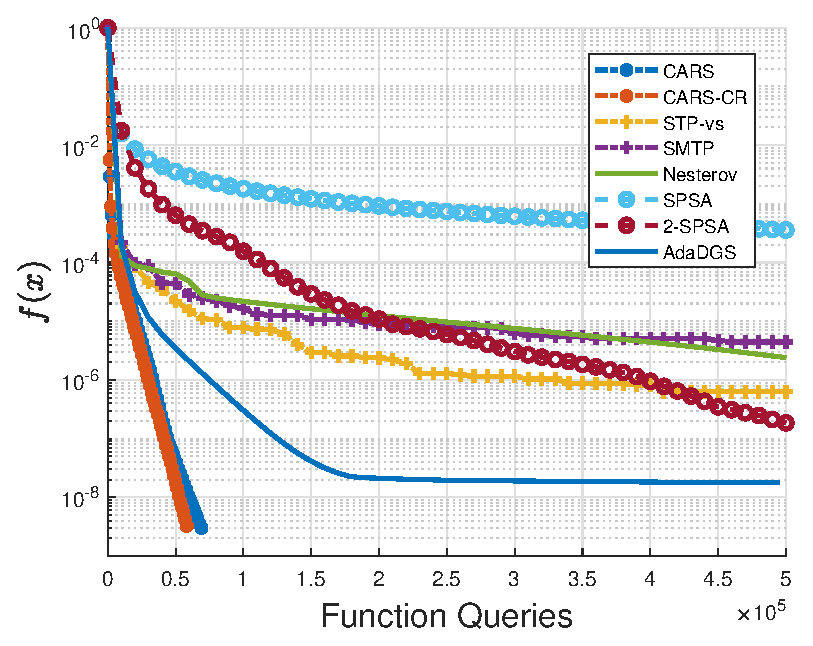
\includegraphics[width=0.8\linewidth]{Quartic_Noiseless_1e-09.eps}
    \caption{Performance of each algorithm on a convex quartic function $f(x) = 0.1\sum_{i=1}^{d} x_i^4 + \frac{1}{2}x^{\top}Ax + 0.01\|x\|^2$, where $A = G^{\top}G$ with $G_{ij} \stackrel{i.i.d}{\sim} \mathcal{N}(0, 1)$. The problem dimension $d = 30$.}
    \label{fig:Convex Quartic}
\end{figure}

\subsection{Benchmark Problem Sets with Non-Convex Functions}
The test results in this section are presented in the form of performance profiles \cite{dolan2002benchmarking}, which is a commonly used tool for comparing the performance of multiple algorithms over a suite of test problems. Performance profiles tend to be more informative than single-dimensional summaries ({\em e.g.} average number of iterations required to solve a problem). Formally, consider fixed sets of problems $\mathcal{P}$ and algorithms $\mathcal{S}$. For each $p \in \mathcal{P}$ and $s \in \mathcal{S}$ the {\em performance ratio} $r_{p,s}$ is defined by
\begin{equation*}
    r_{p,s} = \frac{t_{p,s}}{\min_{s'\in\mathcal{S}} t_{p,s'}},
\end{equation*}
where $t_{p,s}$ is the number of function queries required for $s$ to solve $p$. This is the relative performance of $s$ on $p$ compared to the best algorithm in $\mathcal{S}$ for $p$. The {\em performance profile} of $s$, $\rho_{s} : [1,\infty) \rightarrow [0,1]$ is defined as
\begin{align*}
    \rho_s(\tau) = \frac{|\{p \in \mathcal{P} : r_{p,s} \leq \tau \}|}{|\mathcal{P}|}.
\end{align*}
Therefore, $\rho_s(1)$ is the fraction of problems for which $s$ performs the best, while $\rho_s(\tau)$ for large $\tau$ measures the robustness of $s$. For all $\tau$, a {\em higher value of $\rho_{s}(\tau)$ is better}. We use a log-scale on the horizontal access when plotting $\rho_s(\tau)$.

%\paragraph{Mor\'{e}-Garbow-Hillstrom Problems.}
\vspace{0.1in}
\noindent\textit{\textbf{Mor\'{e}-Garbow-Hillstrom Problems.}}\quad
We tested the same set of algorithms using the well-known non-convex Mor\'{e}-Garbow-Hillstrom 34 test problems \cite{more1981testing}.
For each target accuracy $\varepsilon$, a problem is considered solved when we have $f(x_k)-f_\star \leq \varepsilon(f(x_0)-f_{\star})$ within the budget of 20,000 queries. We used the recommended starting point $x_0$ as in \cite{more1981testing} for all the tested algorithm, and repeated each test 10 times. The results are presented in Figure~\ref{fig:More Garbow Hillstrom and CUTEst}.

%\paragraph{CUTEst Problems.}
\vspace{0.1in}
\noindent\textit{\textbf{CUTEst Problems.}}\quad
We further assessed the performance of CARS and CARS-CR to the same suite of algorithms on the CUTEst \cite{gould2015cutest} problem set, which contains various convex and non-convex problems.
As before, we compared the methods using performance profiles for the 146 problems with dimension less than or equal to 50. The query budget for each problem was set to be $20,000$ times the problem dimension. The target accuracies were again set to $\varepsilon (f(x_0) - f_\star)$. The results are reported in Figure~\ref{fig:More Garbow Hillstrom and CUTEst}.


\begin{figure}
    \centering
    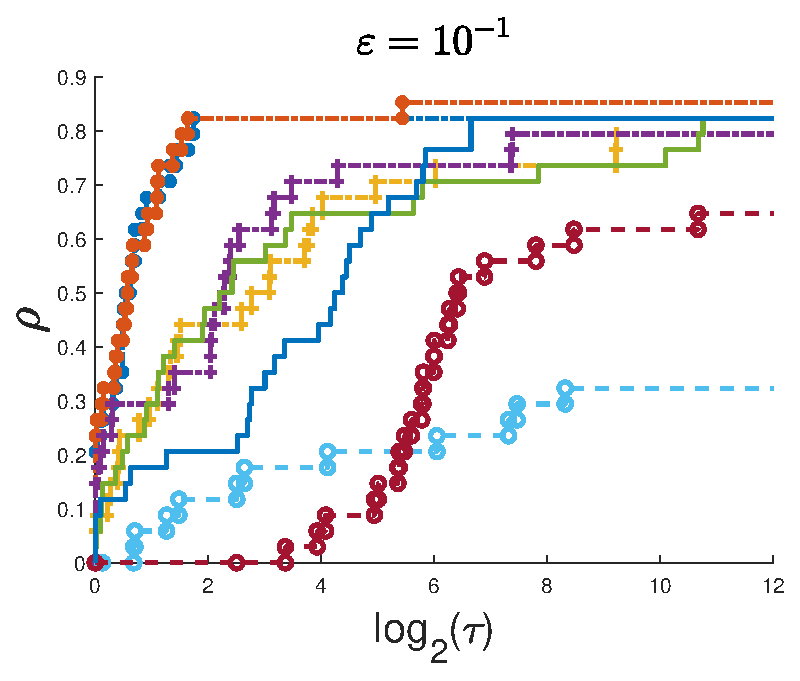
\includegraphics[width=0.4\linewidth]{MORE_perf_prof_1e-01_09-Mar-2023.eps}\qquad
    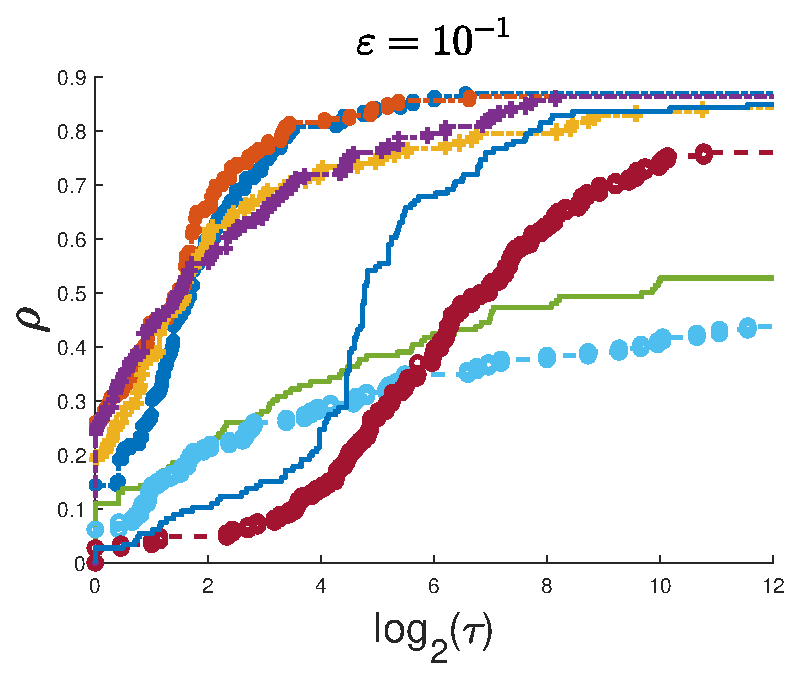
\includegraphics[width=0.4\linewidth]{CUTEst_perf_prof_1e-01_08-Mar-2023.eps} \\
    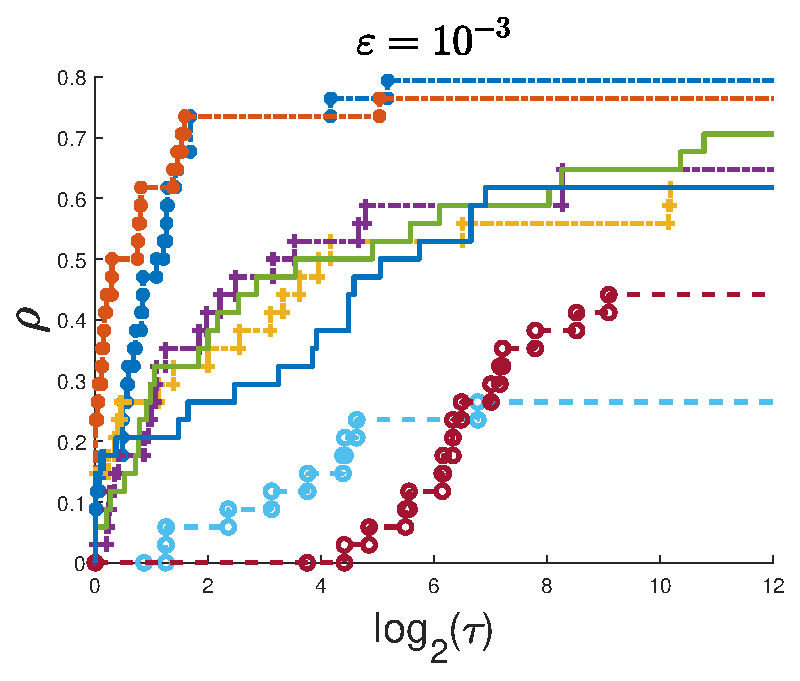
\includegraphics[width=0.4\linewidth]{MORE_perf_prof_1e-03_09-Mar-2023.eps}\qquad
    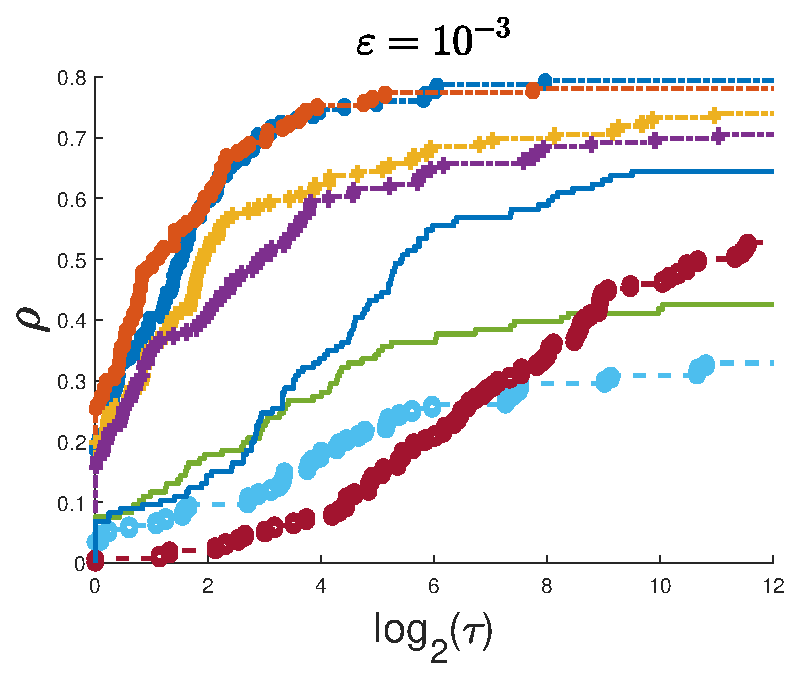
\includegraphics[width=0.4\linewidth]{CUTEst_perf_prof_1e-03_08-Mar-2023.eps} \\
    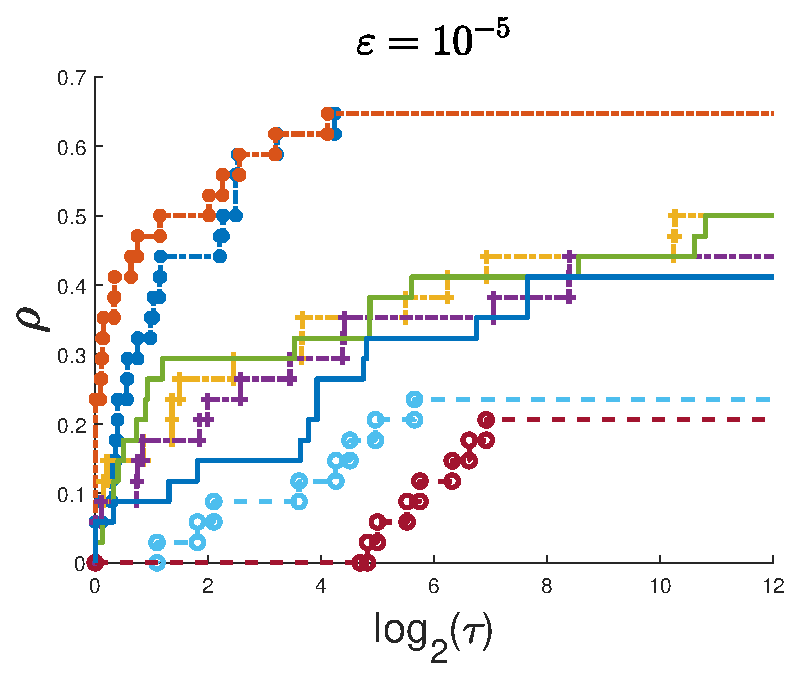
\includegraphics[width=0.4\linewidth]{MORE_perf_prof_1e-05_09-Mar-2023.eps}\qquad
    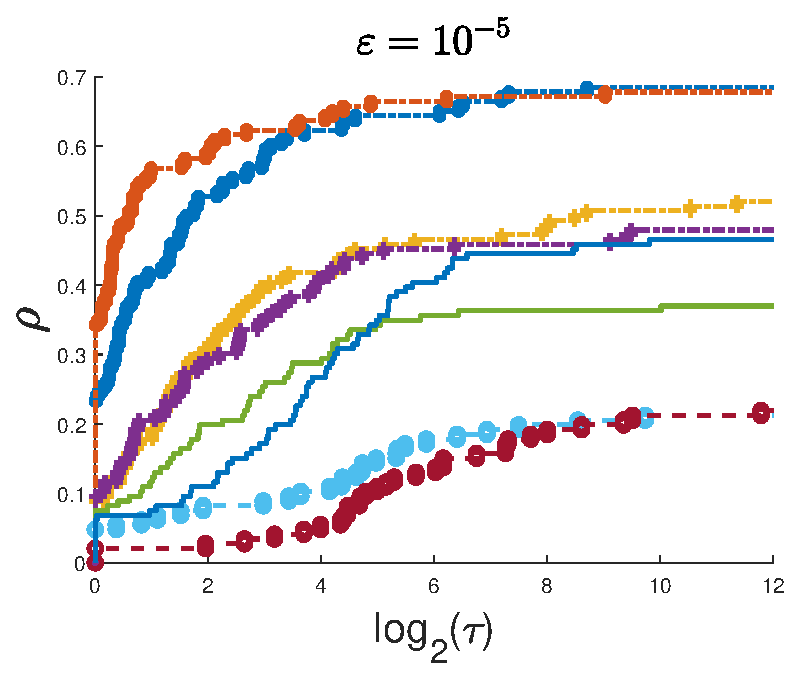
\includegraphics[width=0.4\linewidth]{CUTEst_perf_prof_1e-05_08-Mar-2023.eps}
    \\
    \vspace{5mm}
    {
        \setlength{\fboxsep}{0pt}
        \fbox{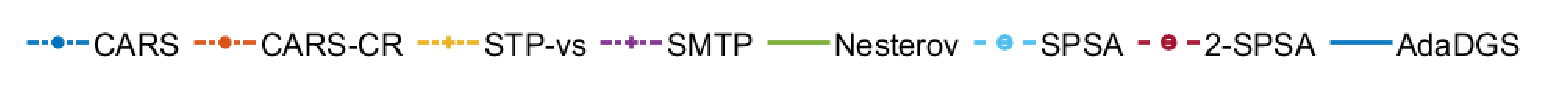
\includegraphics[width=0.8\linewidth]{legend_MORE_all.eps}}
    }\caption{Performance profiles on Mor{\'e}-Garbow-Hillstrom problems (\textbf{left}) and CUTEst problems (\textbf{right}), for various target accuracies $\varepsilon = 10^{-1}$ (\textbf{top}), $10^{-3}$ (\textbf{middle}), and $10^{-5}$ (\textbf{bottom}). Our results demonstrate that CARS and CARS-CR consistently outperform other methods in terms of both efficiency ($\rho$ at low $\tau$ values) and robustness ($\rho$ at high $\tau$ values.) at all levels of accuracy.}\label{fig:More Garbow Hillstrom and CUTEst}
\end{figure}

\subsection{Problems with Highly Oscillatory Noise}
We also evaluated the performance of the algorithms, including CARS-NQ, on the same set of problems, but this time with additional highly oscillatory noise. The results are depicted in Figure~\ref{fig:Convex Quartic with Noise}.
The experiment notably showcases the efficacy of an increased sampling radius for CARS-NQ.
\begin{figure}
    \centering
    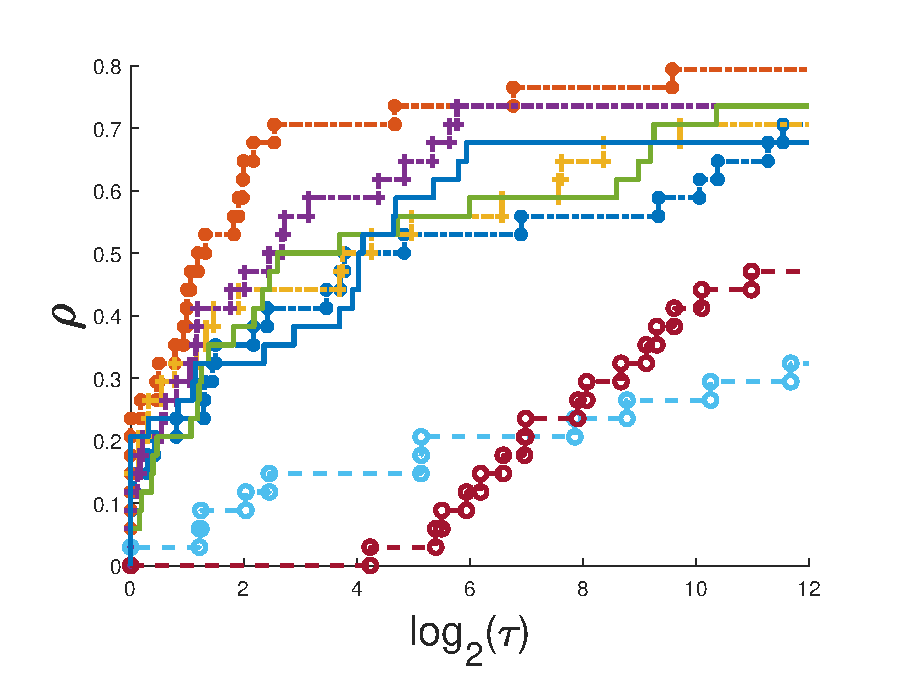
\includegraphics[width=0.8\linewidth]{Osc_MORE_ALL_EPS_1e-3_noise_0.05EPS.eps}
    \vspace{1mm}
    {
        {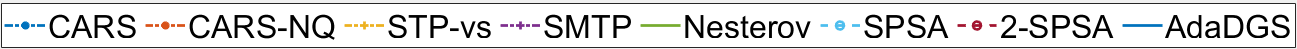
\includegraphics[width=0.8\linewidth]{MORE_ALL_LEGEND.png}}
    }
    \caption{Performance of each algorithm on Mor\'{e}-Garbow-Hillstrom Problems with sinusoidal noise $f_{\mathrm{osc}}(x) = \psi \frac{1}{d}\sum_{i=1}^{d}(1-\cos(\phi x_i))$, where  $\psi = 0.05\varepsilon(f(x_0)-f_\star)$ and $\phi = 100\pi$. The target accuracy $\varepsilon$ is set to $10^{-3}$.}
    \label{fig:Convex Quartic with Noise}
\end{figure}



\subsection{Black-box Adversarial Attacks}
\begin{table}[t]
    \centering
    \def\ROWCOLOR{black!10!white}
    \begin{tabular}{l c c c}
        \toprule
        Algorithm      & Success Rate (\%) & Median Queries & Average Queries \\
        \midrule
        \rowcolor{\ROWCOLOR}
        ZOO$^*$        & 93.95             & 11,700         & 11,804          \\
        PGD-NES$^*$    & 88.39             & 2,450          & 4,584           \\
        \rowcolor{\ROWCOLOR}
        ZOHA-Gauss$^*$ & 91.69             & 1,400          & 2,586           \\
        ZOHA-Diag$^*$  & 91.06             & 1,656          & 3,233           \\
        \rowcolor{\ROWCOLOR}
        STP            & 53.64             & 2,193          & 3,141           \\
        SMTP           & 65.68             & 1,415          & 2,250           \\
        \rowcolor{\ROWCOLOR}
        Nesterov       & 67.72             & 1,105          & 2,044           \\
        Square Attack  & \textbf{98.21}   & 1,060          & 1,297           \\
        \rowcolor{\ROWCOLOR}
        CARS (Square)  & 97.09             & \textbf{717}  & \textbf{1,169} \\
        \bottomrule
    \end{tabular}
    \caption{Comparison of success rates, and median and average function queries for the successful black-box adversarial attacks on MNIST with $\ell_\infty$-perturbation bound 0.2.
        CARS, equipped with the Square Attack's distribution, shows the best performance in successful attacks, while reaching the second best success rate. The results marked with $^*$ are cited from \cite{ye2018hessian}.
    }
    \label{table: Black Box Attack to a CNN model on the MNIST dataset}
\end{table}
Suppose $\mathcal{N}$ is an image classifier.
The problem of generating small perturbations $x$ that, when added to a natural image $x_{\mathrm{nat}}$, fool the classifier ({\em i.e.} $\mathcal{N}(x_{\mathrm{nat}} + x) \neq \mathcal{N}(x_{\mathrm{nat}})$) is known as finding an {\em adversarial attack} \cite{goodfellow2014explaining}. As described in \cite{chen2017zoo}, when no access to the internal workings of the classifier
is available, this problem becomes a black-box, or derivative-free, optimization problem. In order to ensure the attacked image $x_{\mathrm{nat}} + x$ appears natural, a pixel-wise bound $\|x\|_{\infty} \leq \varepsilon_{\mathrm{atk}}$ is usually enforced. CARS showed state-of-the-art performance in generating black-box adversarial attacks for $\mathcal{N}$ trained on the MNIST digit classification dataset \cite{lecun2010mnist}.

In our experiments, $\mathcal{N}$ is a two-layer CNN achieving $99\%$ test accuracy on unperturbed images. We use $\varepsilon_{\mathrm{atk}} = 0.2$ and consider all $10,000$ images from the test set of MNIST. We consider an attack a success if it fools $\mathcal{N}$ before a budget of $10,000$ queries is met. The success rates, median and average queries for successful attacks are shown in Table~\ref{table: Black Box Attack to a CNN model on the MNIST dataset}.
The results from ZOO \cite{chen2017zoo}, PGD-NES \cite{ilyas2018black}, and ZOHA-type algorithms \cite{ye2018hessian} are cited from \cite{ye2018hessian}.
As pointed out in Section~\ref{section:convergence of CARS}, the choice of sampling directions for CARS is not restrictive. Hence we used a similar initialization and distribution $\mathcal{D}$ as the Square Attack \cite{andriushchenko2020square}, which is known to be particularly well-suited for attacking CNN models.
Visualization of attacked images is partly shown in Figure~\ref{fig:MNIST_ATK_RES}. More pictures and detailed settings can be found in Appendix~\ref{appendix: Experiments}.

\begin{figure}
    \centering
    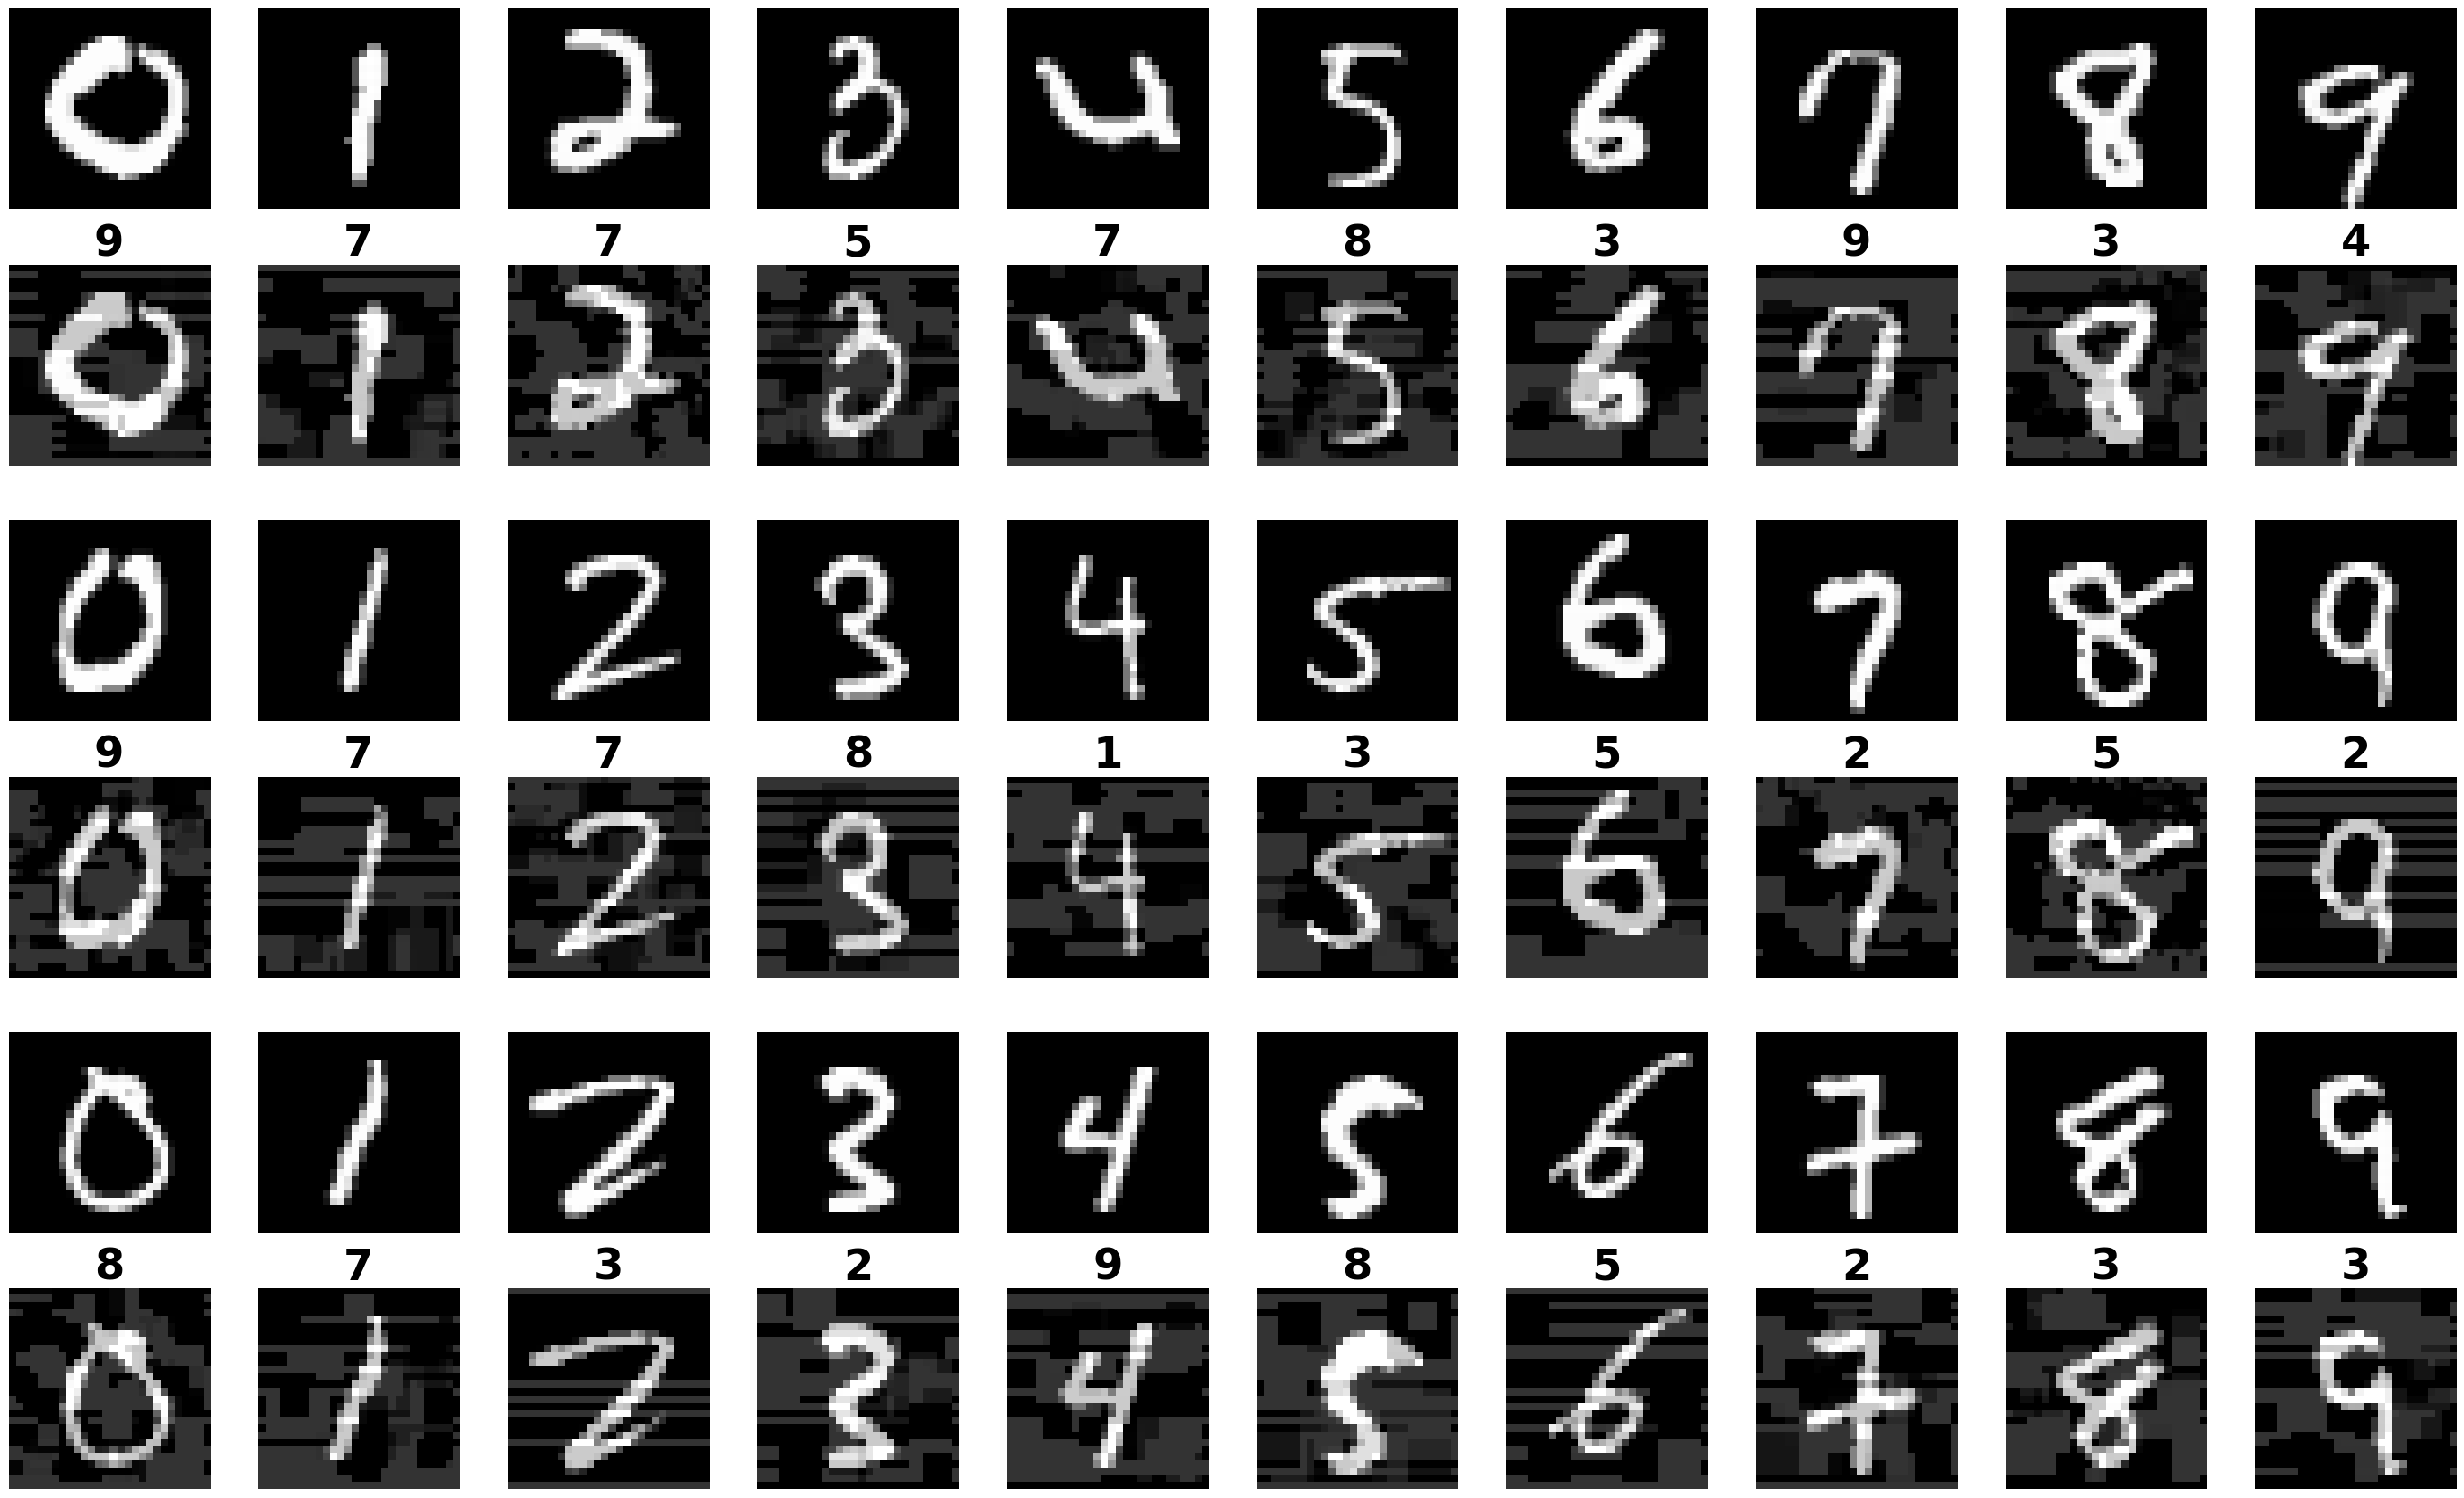
\includegraphics[width=0.8\linewidth]{MNISTatk_imgs_horizontal_60_B.eps}
    \caption{Adversarial examples with misclassified labels on MNIST generated with CARS. More pictures are available in Appendix~\ref{appendix: Experiments}.}
    \label{fig:MNIST_ATK_RES}
\end{figure}

\subsection{Benchmarking the Performance of SHIPS}
In this section we present a numerical result for SHIPS, which is a combination of CARS and the randomized matrix inversion presented in Section~\ref{section:SHIPS}. The main purpose of this comparison is to assess SHIPS' ability to generate effective search directions. Thus, we contrast it with Exact Gradient Descent (Exact GD), and variance-reduced version of CARS and Nesterov-Spokoiny (CARS-VarRed and NS-VarRed, respectively.) 

For a fairer comparison with methods based on exact derivatives, we, in the case of DFO methods, sample $d$ directions and use $2d$ queries to estimate the directional derivatives per iteration.

Variance reduction, achieved by utilizing multiple samples when calculating the expectation, has shown to work well for Nesterov-Spokoiny \cite{salimans2017evolution,mania2018simple}.
In contrast, CARS, does not have a known reduced variance version yet. For this, we apply a multi-sample extension \eqref{eq: ES extension of CARS multiple samples} as introduced in Section~\ref{section: connection to ES}.

The test function for our benchmark is given by:
\begin{equation}
    f(x) = \frac{1}{2}x^{\top}A x + \frac{1}{12} \sum_{i=1}^{d} \alpha_{i} x_{i}^{4},
\end{equation}
where $A$ is a random positive definite matrix with $A = G^{\top}G$ with $G_{ij} \stackrel{i.i.d}{\sim} \mathcal{N}(0, 1)$, and $\alpha_i \stackrel{i.i.d}{\sim} \unif(0, 1)$.

For each iteration, we used $d$ uniformly random directions on the unit sphere, and consumed $2d$ queries to estimate the respective directional derivatives. 
The methods labeled \emph{Exact GD} and \emph{Exact SHIPS} are provided with the exact gradient and Hessian for comparative purposes.
As demonstrated in Figure~\ref{fig:SHIPS_vs_others}, SHIPS deivers superior convergence speed.

\begin{figure}
    \centering
    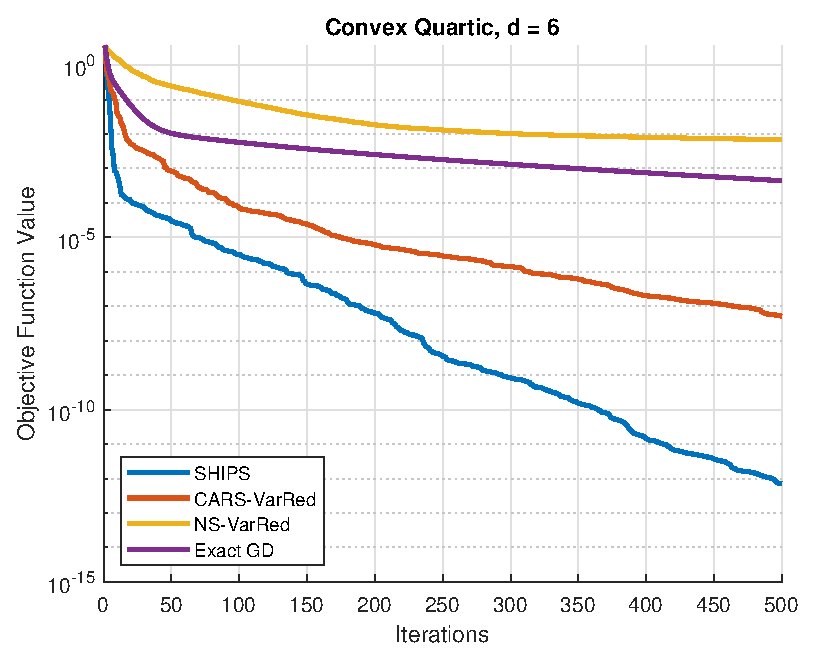
\includegraphics[width=0.8\linewidth]{SHIPS_vs_others.eps}
    \caption{The $x$-axis denotes the number of iterations, not the number of function queries. Among all the methods, SHIPS shows the best convergence rate,  outperforming even Exact GD, as it effectively utilizes the curvature information.}
    \label{fig:SHIPS_vs_others}
\end{figure}